\documentclass[aspectratio=169]{beamer}
\usepackage{ctex}
\usepackage{graphicx}
\usepackage{hyperref}

\usetheme{Madrid}
\setbeamertemplate{navigation symbols}{}
\graphicspath{{./}{./papers/}}

\title{个人简介与论文工作汇报}
\author{侯健}
\institute{中国人民大学统计学院}
\date{2026年2月}

\begin{document}

\begin{frame}
  \titlepage
\end{frame}

\section{个人信息}

\begin{frame}[t]{个人简介}
  \begin{columns}[T,onlytextwidth]
    \column{0.34\textwidth}
      \centering
      \includegraphics[width=\linewidth]{hj.jpg}
    \column{0.66\textwidth}
      \small
      \begin{itemize}
        \item 统计学在读博士 | 初级统计师
        \item 研究方向:分位回归、鞍点逼近、混合效应建模
        \item 机构:中国人民大学统计学院
        \item 邮箱:\href{mailto:houjian1997@ruc.edu.cn}{houjian1997@ruc.edu.cn}
        \item ORCID:\href{https://orcid.org/0000-0002-9248-6874}{0000-0002-9248-6874}
        \item GitHub:\href{https://github.com/Stork343}{Stork343}
      \end{itemize}
  \end{columns}
\end{frame}

\begin{frame}[t]{研究领域与合作}
  \small
  \begin{itemize}
    \item 分位回归:高维分位回归建模、混合效应数据的非光滑估计与渐近推断。
    \item 鞍点逼近:半参数鞍点逼近方法、区间估计与数值优化。
    \item 混合效应:纵向数据分析、大规模全基因组关联分析与可扩展贝叶斯/变分方法。
    \item 主要合作者:TIAN Maozai,MENG Tan,WANG Zhihao。
    \item 地址:北京市海淀区中关村大街59号,中国人民大学。
  \end{itemize}
\end{frame}

\section{论文工作}

\begin{frame}[t]{基于 Mallows 模型的大语言模型特征排序校准方法}
  \begin{columns}[T,onlytextwidth]
    \column{0.62\textwidth}
      \footnotesize
      \textbf{作者:} 侯健,田茂再\\
      \textbf{期刊:} 统计研究\\
      \textbf{工作要点:}
      \begin{itemize}
        \item 构建 Mallows 排序模型,对大语言模型输出的特征重要性排序进行统计校准。
        \item 提出排序一致性度量与估计流程,验证校准效果与收敛性。
      \end{itemize}
    \column{0.38\textwidth}
      \centering
      \includegraphics[width=\linewidth]{papers/2025/mallows-llm-ranking/fig_estimation_convergence.png}
  \end{columns}
\end{frame}

\begin{frame}[t]{Jointly Penalised and Debiased Inference\\for High-Dimensional Mixed Effects Quantile Regression}
  \begin{columns}[T,onlytextwidth]
    \column{0.62\textwidth}
      \footnotesize
      \textbf{作者:} Hou Jian, Meng Tan, Tian Maozai\\
      \textbf{期刊:} Statistica Sinica\\
      \textbf{工作要点:}
      \begin{itemize}
        \item 提出联合惩罚的高维混合效应分位回归估计,实现固定效应选择与随机效应估计。
        \item 基于去偏技术构造统计推断,给出置信区间与显著性检验。
      \end{itemize}
    \column{0.38\textwidth}
      \centering
      \includegraphics[width=\linewidth]{papers/2025/jpdi-mixed-qr/dblqmm.png}
  \end{columns}
\end{frame}

\begin{frame}[t]{Sparse-Smooth Spatially Varying Coefficient\\Quantile Regression}
  \begin{columns}[T,onlytextwidth]
    \column{0.62\textwidth}
      \footnotesize
      \textbf{作者:} Hou Jian, Meng Tan, Tian Maozai\\
      \textbf{期刊:} arXiv/Spatial Statistics(1st revision)\\
      \textbf{工作要点:}
      \begin{itemize}
        \item 构建稀疏-平滑的空间变系数分位回归模型,实现变量选择与空间平滑。
        \item 在房价数据中捕捉空间异质性,提升解释性与预测精度。
      \end{itemize}
    \column{0.38\textwidth}
      \centering
      \includegraphics[width=\linewidth]{papers/2025/svcqr/SVCQR.png}
  \end{columns}
\end{frame}

\begin{frame}[t]{Hierarchical Composite Quantile Regression\\with Adaptive Lasso}
  \begin{columns}[T,onlytextwidth]
    \column{0.62\textwidth}
      \footnotesize
      \textbf{作者:} Hou Jian, Meng Tan, Tian Maozai\\
      \textbf{期刊:} Journal of Statistical Planning and Inference(1st revision)\\
      \textbf{工作要点:}
      \begin{itemize}
        \item 提出层级复合分位回归与自适应 Lasso,处理高维固定效应和重尾误差。
        \item 采用 EM + ADMM 的估计流程,同时估计随机效应与方差分量。
      \end{itemize}
    \column{0.38\textwidth}
      \centering
      \includegraphics[width=\linewidth]{"papers/2025/hcqr/data-line.png"}
  \end{columns}
\end{frame}

\begin{frame}[t]{Self-Normalized Quantile Empirical\\Saddlepoint Approximation}
  \begin{columns}[T,onlytextwidth]
    \column{0.62\textwidth}
      \footnotesize
      \textbf{作者:} Hou Jian, Meng Tan, Tian Maozai\\
      \textbf{期刊:} arXiv/Statistical Papers(Under Review)\\
      \textbf{工作要点:}
      \begin{itemize}
        \item 提出自标准化分位经验鞍点逼近,提高小样本推断精度。
        \item 构造更短且覆盖率更高的置信区间,并在模拟中验证优势。
      \end{itemize}
    \column{0.38\textwidth}
      \centering
      \includegraphics[width=\linewidth]{papers/2025/snqesa/spx_plots.png}
  \end{columns}
\end{frame}

\begin{frame}[t]{部分线性地理加权分位回归模型}
  \begin{columns}[T,onlytextwidth]
    \column{0.62\textwidth}
      \footnotesize
      \textbf{作者:} 侯健,刘硕,田茂再\\
      \textbf{期刊:} 应用数学学报(外审)\\
      \textbf{工作要点:}
      \begin{itemize}
        \item 构建部分线性 GWR 分位回归模型,允许部分协变量局部变化。
        \item 在空间数据中兼顾全局趋势与局部效应,提升解释能力。
      \end{itemize}
    \column{0.38\textwidth}
      \centering
      \includegraphics[width=\linewidth]{papers/2025/plgwqr/plgwqr.png}
  \end{columns}
\end{frame}

\begin{frame}[t]{泊松分布下基于鞍点逼近的\\相对风险置信区间构造}
  \begin{columns}[T,onlytextwidth]
    \column{0.62\textwidth}
      \footnotesize
      \textbf{作者:} 侯健,刘硕,田茂再\\
      \textbf{期刊:} 统计与信息论坛(2025)\\
      \textbf{工作要点:}
      \begin{itemize}
        \item 在泊松分布假设下推导鞍点逼近的相对风险置信区间公式。
        \item 通过蒙特卡洛与实证分析验证区间更短、覆盖率更接近名义水平。
      \end{itemize}
    \column{0.38\textwidth}
      \centering
      \includegraphics[width=\linewidth]{papers/2025/poisson-rr/poisson-rr.jpeg}
  \end{columns}
\end{frame}

\begin{frame}[t]{基于异窗宽 GTWR 模型的\\商品住宅价格影响因素研究}
  \begin{columns}[T,onlytextwidth]
    \column{0.62\textwidth}
      \footnotesize
      \textbf{作者:} 侯健,王芝皓,田茂再,窦燕\\
      \textbf{期刊:} 数理统计与管理(2022)\\
      \textbf{工作要点:}
      \begin{itemize}
        \item 提出异窗宽 GTWR 模型与标准差椭圆加权算法,降低计算量。
        \item 揭示交通便利性和绿化率对房价的时空异质影响。
      \end{itemize}
    \column{0.38\textwidth}
      \centering
      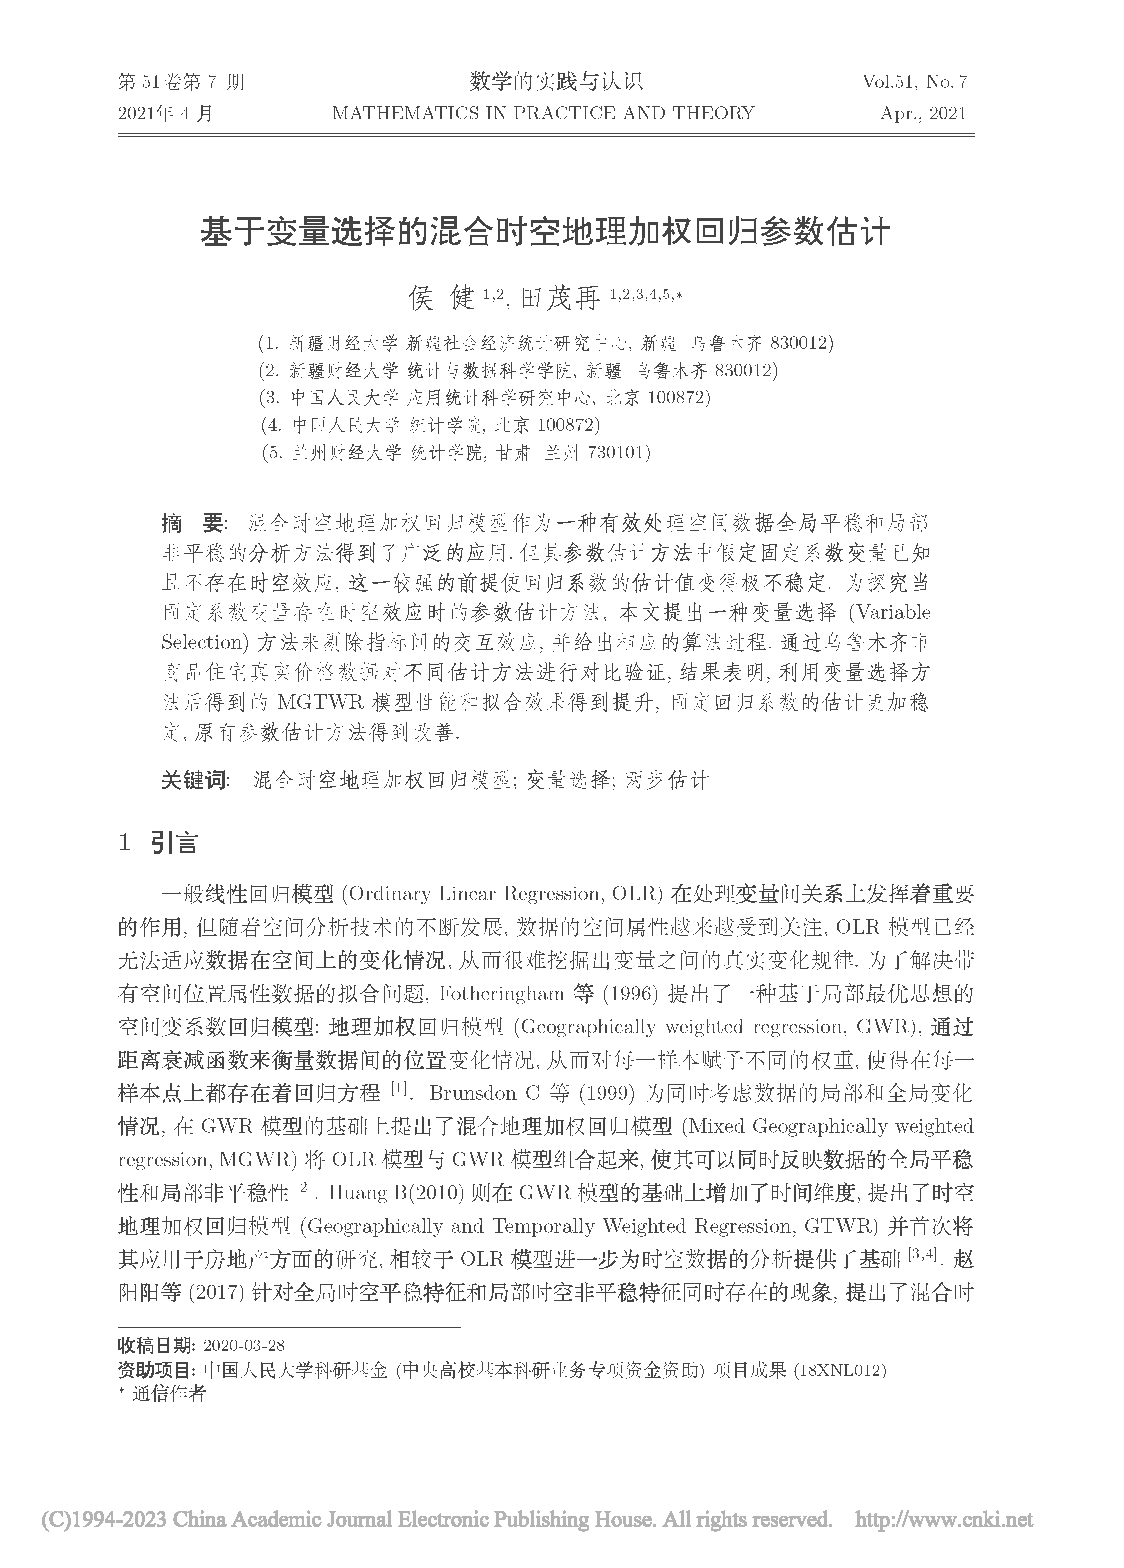
\includegraphics[width=\linewidth]{papers/2022/gtwr-housing/mgtwr.png}
  \end{columns}
\end{frame}

\begin{frame}[t]{基于多尺度时空地理加权回归模型的\\房价影响因素分析}
  \begin{columns}[T,onlytextwidth]
    \column{0.62\textwidth}
      \footnotesize
      \textbf{作者:} 景昊坤,王合玲,侯健\\
      \textbf{期刊:} 统计与管理(2022)\\
      \textbf{工作要点:}
      \begin{itemize}
        \item 构建多尺度时空地理加权回归模型(MGCTWR)分析房价空间异质性。
        \item 对比 GTWR 模型并识别区位、绿化率等关键影响因素。
      \end{itemize}
    \column{0.38\textwidth}
      \centering
      \includegraphics[width=\linewidth]{papers/2022/bgtwr-housing/bgtwr.png}
  \end{columns}
\end{frame}

\begin{frame}[t]{基于变量选择的混合时空地理加权回归\\参数估计}
  \begin{columns}[T,onlytextwidth]
    \column{0.62\textwidth}
      \footnotesize
      \textbf{作者:} 侯健,田茂再\\
      \textbf{期刊:} 数学的实践与认识(2021)\\
      \textbf{工作要点:}
      \begin{itemize}
        \item 提出变量选择方法处理固定系数变量的时空效应,提高估计稳定性。
        \item 在乌鲁木齐房价数据中验证 MGTWR 参数估计的改进效果。
      \end{itemize}
    \column{0.38\textwidth}
      \centering
      \includegraphics[width=\linewidth]{papers/2021/mgtwr-variable-selection/gtwr.png}
  \end{columns}
\end{frame}

\begin{frame}
  \centering
  \Huge 谢谢!
\end{frame}

\end{document}
